\documentclass[conference]{IEEEtran}
\IEEEoverridecommandlockouts
\usepackage{hyperref}
\hypersetup{
    colorlinks=true, linkcolor=blue, filecolor=magenta, urlcolor=blue, citecolor=blue}

% The preceding line is only needed to identify funding in the first footnote. If that is unneeded, please comment it out.
\usepackage{cite}
\usepackage{bookmark}
\usepackage{amsmath,amssymb,amsfonts}
\usepackage{algorithmic}
\usepackage{graphicx}
\usepackage{textcomp}
\usepackage{xcolor}
\def\BibTeX{{\rm B\kern-.05em{\sc i\kern-.025em b}\kern-.08em
    T\kern-.1667em\lower.7ex\hbox{E}\kern-.125emX}}

\usepackage{setspace}

\onehalfspacing
\begin{document}

\title{Multi-Task Learning for Stock Price Prediction \\ [1ex] \large Computational Intelligence (CIS*4780) - March 2026}
\date{March 2026}

\author{\IEEEauthorblockN{Stella Rovazzi \\ srovazzi@uoguelph.ca}
\and
\IEEEauthorblockN{Matthew Lawford \\ mlawford@uoguelph.ca}
\and
\IEEEauthorblockN{Julia Horner \\ jhorne03@uoguelph.ca}}


\maketitle

%---------------------------------------ABSTRACT-------------------------------------
\section*{Abstract}
**Insert abstract here**

%--------------------------------------INTRODUCTION-------------------------------------
\section{Introduction}
**Insert introduction here**

%-------------------------------------MOTIVATION and OBJECTIVES------------------------
\section{Motivation and Objectives}
\subsection*{Motivation}
\subsection*{Objectives}

%-------------------------------------METHODOLOGY-------------------------------------
\section{Methodology}
\subsection{Data}
- Companies \\
- aggregation choice \\
- time choice \\

\subsection{Algorithms}
\subsubsection*{Random Forests}
yee
\subsubsection*{LSTMS}
explination
\begin{figure}[h]
    \centering
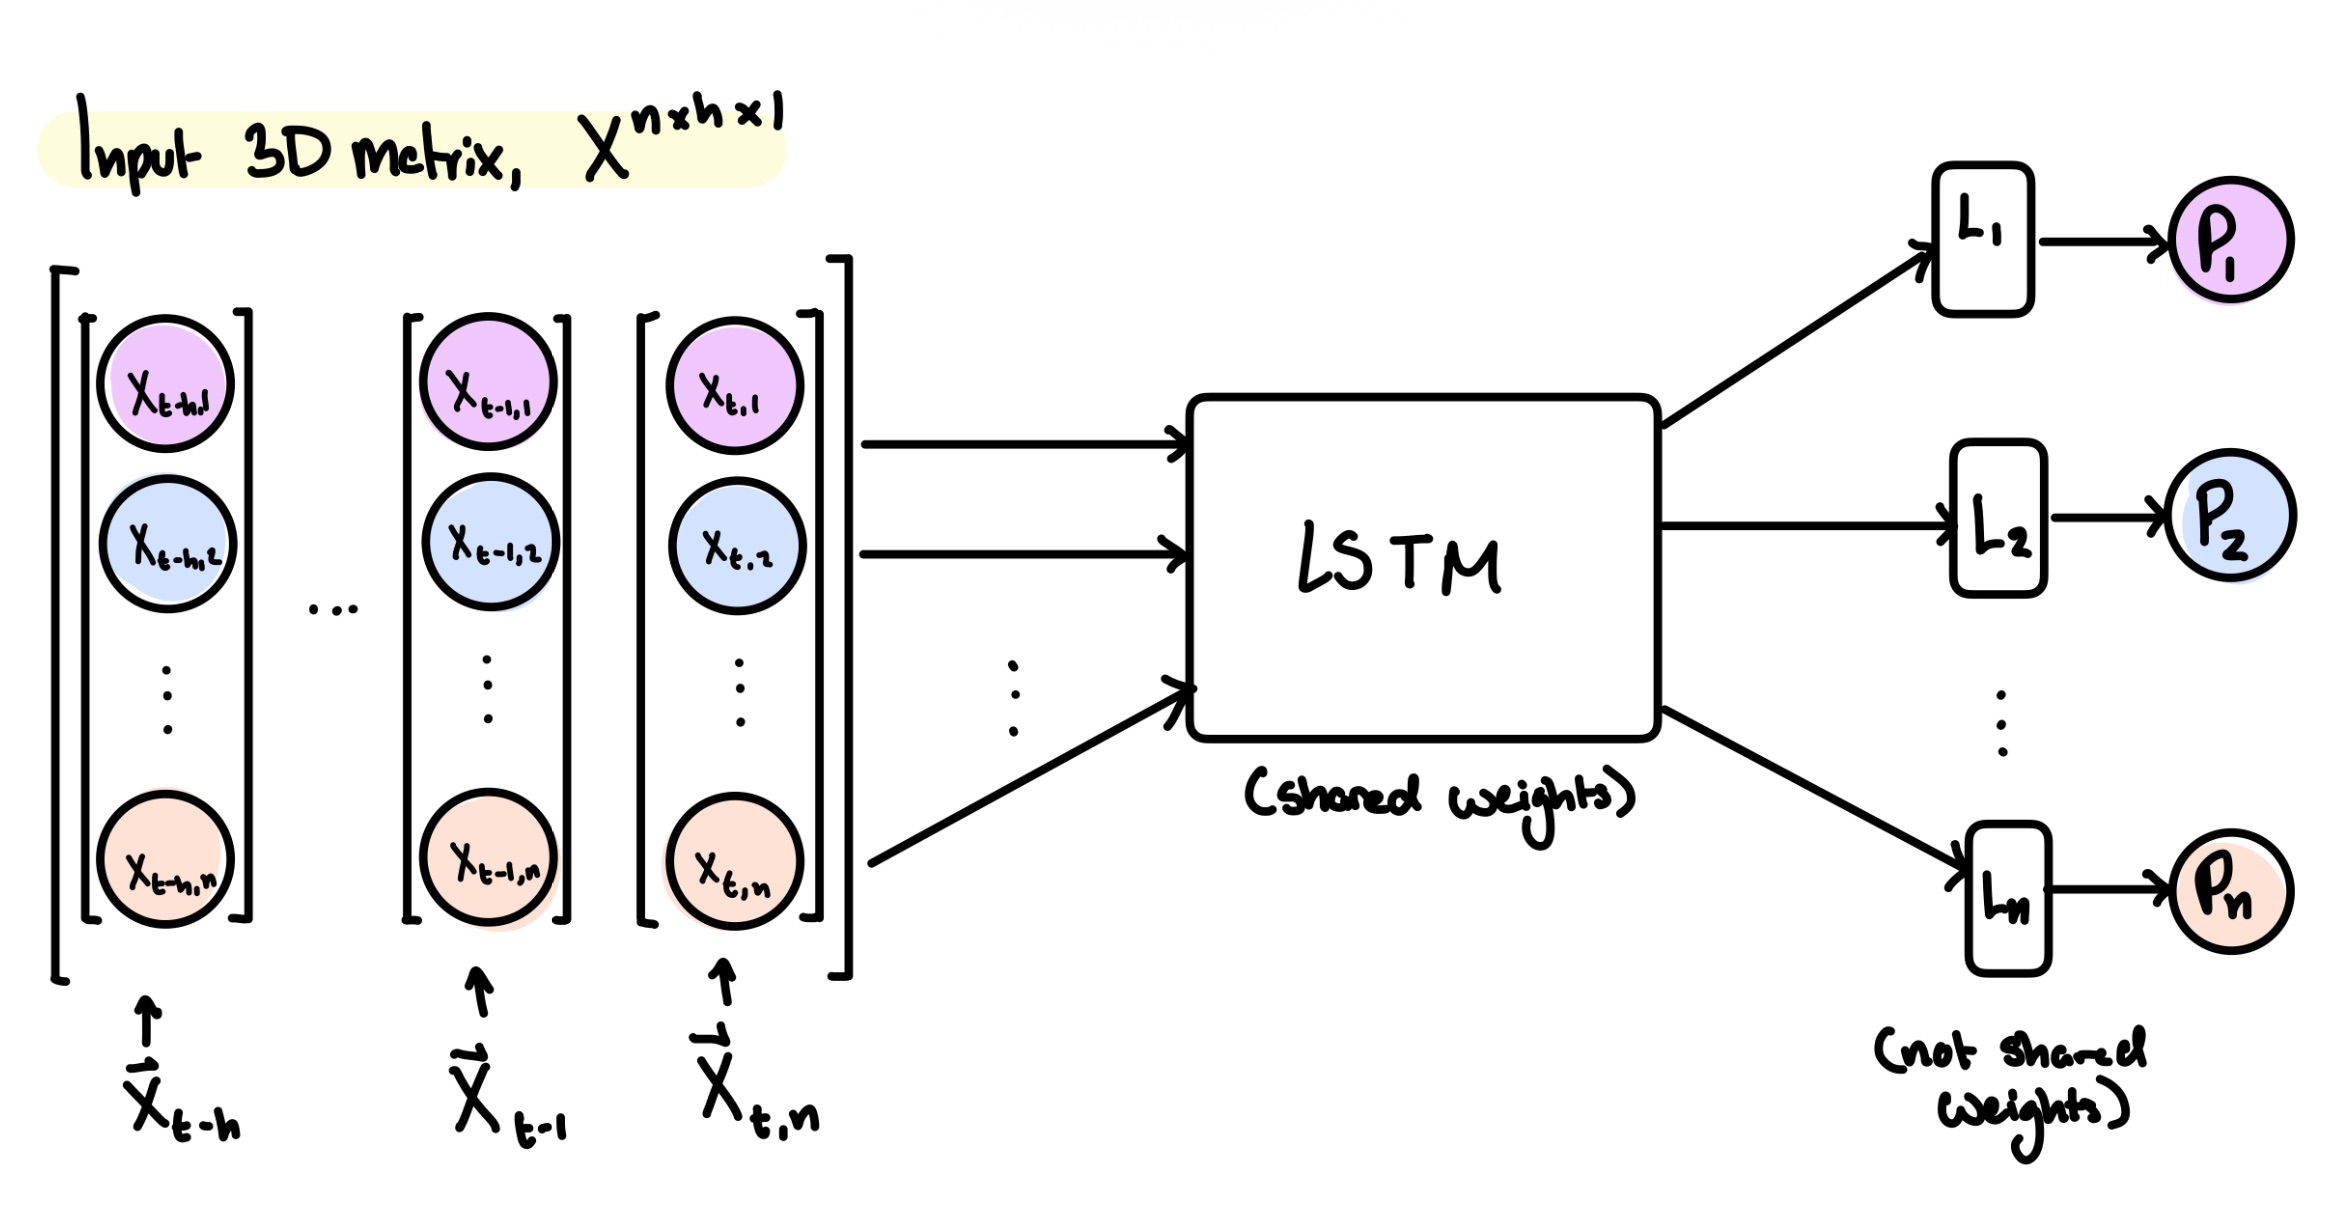
\includegraphics[width=0.7\linewidth]{images/lstm_inputs.png}
    \caption{Diagram of hard parameter sharing and inputs for an LSTM Multi-Tasking model. (Drawn by group).}
    \label{lstm_diagram}
\end{figure}

\subsection{Metrics and Evaluation}

\subsection{Preprocessing}
\subsubsection*{Misaligned Dates}
Due to different market holidays, some days in the data included both null values and
 recorded prices. The days with null values were removed to keep the dataset consistent.
  Dropping a few days of data should not obscure the stocks’ growth patterns and relationships.
\subsubsection*{Logarithmic Scale}
The data was scaled logarithmically. This was to ensure stable predictions by reducing 
 effect of outliers on the model and to account for the exponential patterns in each stock's data.
The predictions become more stable because most analysis techniques assume additive data, including
machine learning.\cite{log_scale}. \\
The scaling affect is shown in appendix \ref{appendix_a}, the medium stock ACIW is on a similar scale to the large 
stock AAPL after logging the data.

\subsubsection*{Random Forests}
describe script and set up of what it intakes \cite{log_scale}
\subsubsection*{LSTMS}
Pytorch requires LSTM inputs to be 3D tensors. The data looks at stocks, with the only attribute 
being the stock price. Referring to \ref{lstm_diagram}, the matrix on the left would be an example 3D tensor input,
with each vector $\vec{x}$ representing all the stocks of interest at the given t. There is no third dimension depicted,
as the only attribute of each stock of interest is the given price at time t. \\
The times within the input are $\vec{x_{t,n}}$ and the lags of $\vec{x_{tn}}$, which represent our rolling window,
 since $\vec{x_{t+1}}$ should use all the previous lags for its prediction.

\subsection{Building the Models (?)}
\subsubsection*{Random Forests}
\subsubsection*{LSTMS}

%---------------------------------------RESULTS-------------------------------------
\section{Results}
*add pics and stuff*
\subsection{Hyperparameters}
\subsection{Algorithm Performances}

%---------------------------------------DISCUSSIONS-------------------------------------
\section{Discussion}
\subsection{Findings}
\subsection{Interpretation of Results}
\subsection{Hyperparameters}
\subsection{Advantages and Disadvantages of Multi-Tasking}

%--------------------------------------CONCLUSION-------------------------------------
\section{Conclusion}

%-------------------------------------BIBLIOGRAPHY-------------------------------------
\bibliographystyle{IEEEtran}
\bibliography{refs}


%------------------------------------APPENDIX-----------------------------------------
\appendix
\counterwithin{figure}{section} % Resets figure count to 0, prefixes with section letter (A, B, etc.)
\renewcommand{\thefigure}{\thesection\arabic{figure}} % Formats as A1 instead of A.1
\section{Raw Data}
\label{appendix_a}
\begin{figure}[h]
    \centering
    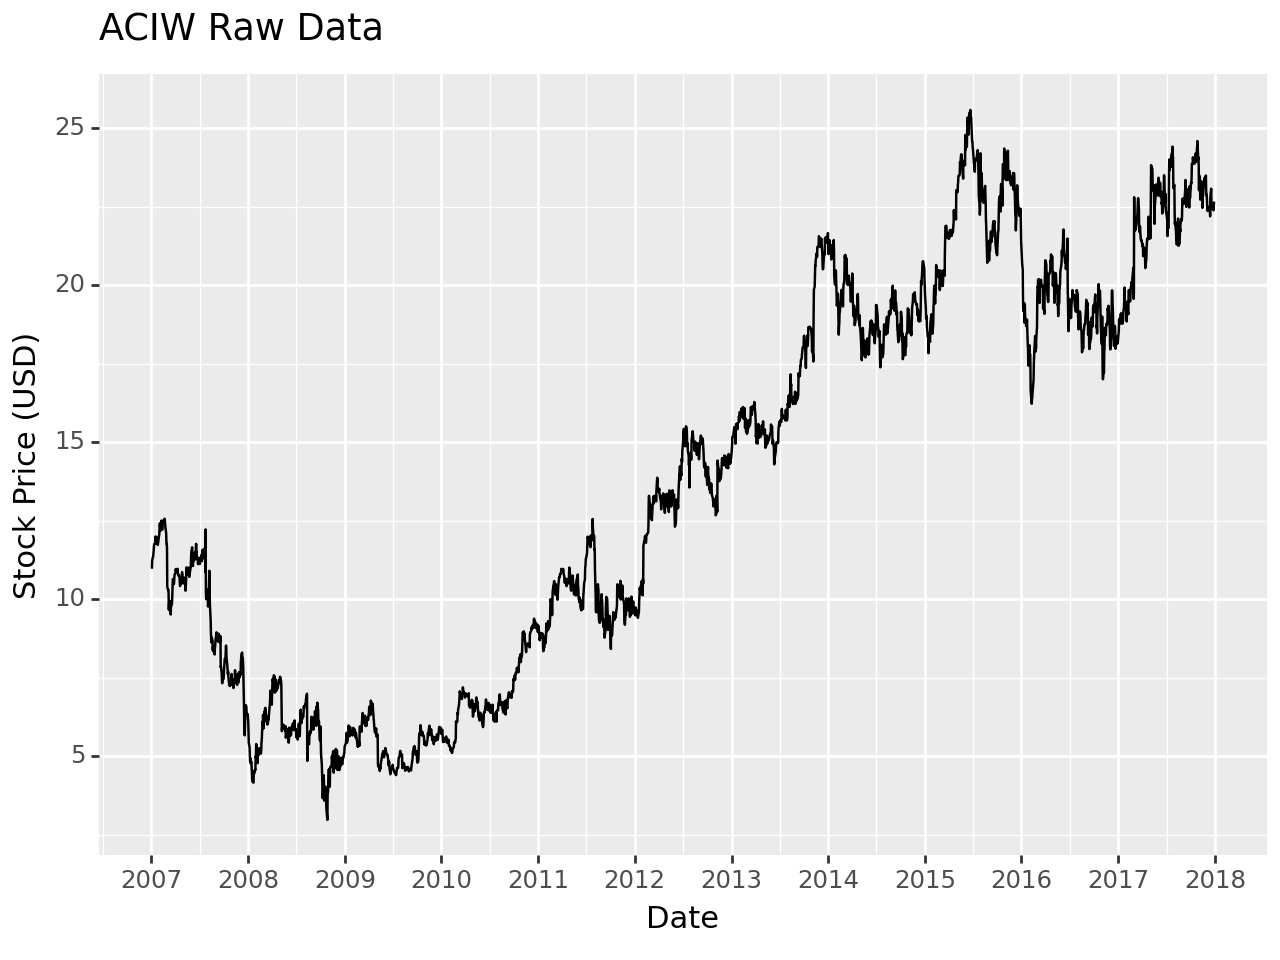
\includegraphics[width=0.7\linewidth]{images/aciw_raw.png}
    \caption{Raw price data of ACIW Stock}
    \label{aciw_raw}
\end{figure}

\begin{figure}[h]
    \centering
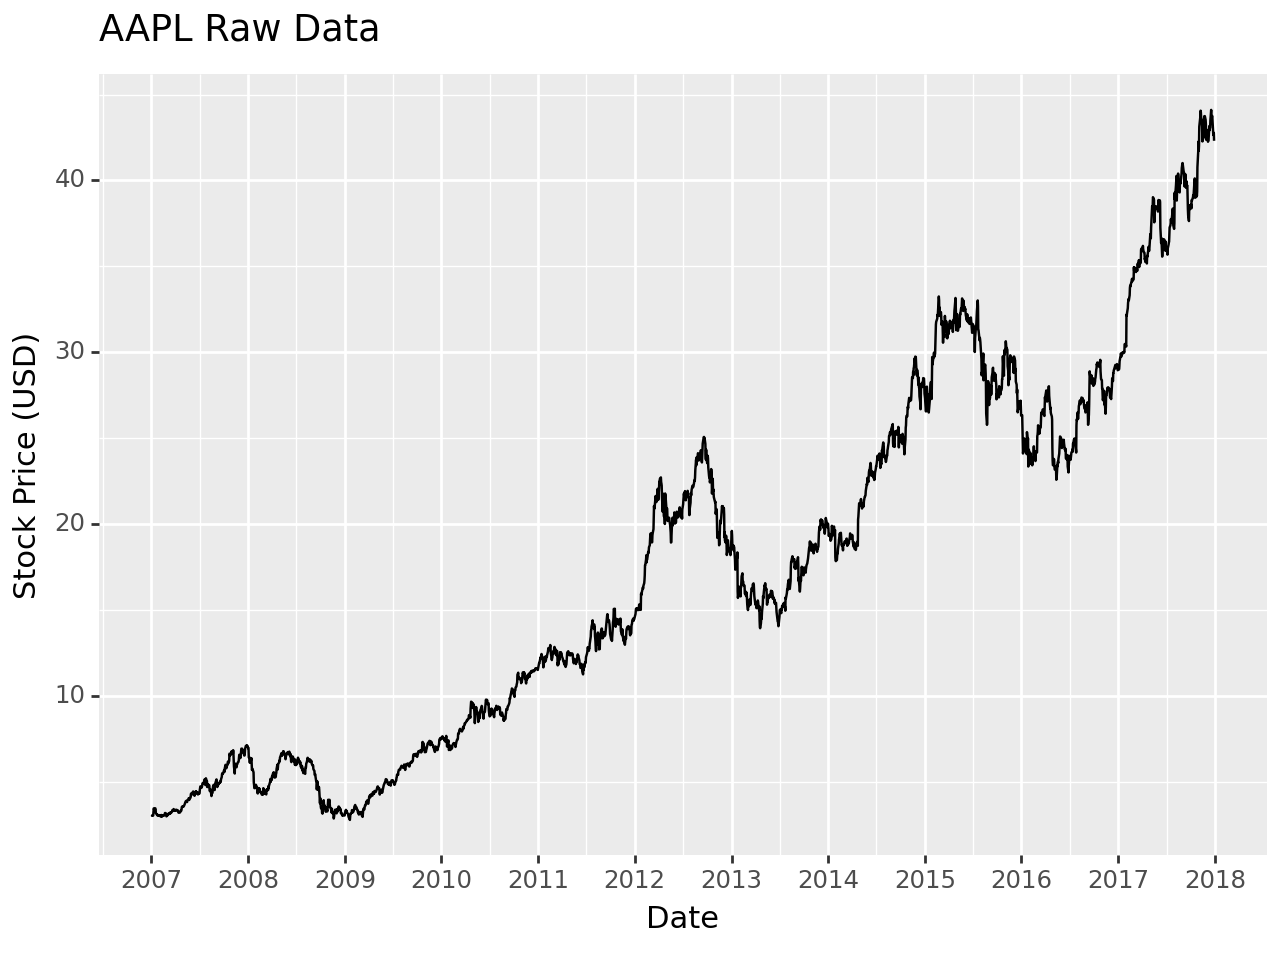
\includegraphics[width=0.7\linewidth]{images/appl_raw.png}
    \caption{Raw price data of APPL Stock}
    \label{appl_raw}
\end{figure}

\begin{figure}[h]
    \centering
    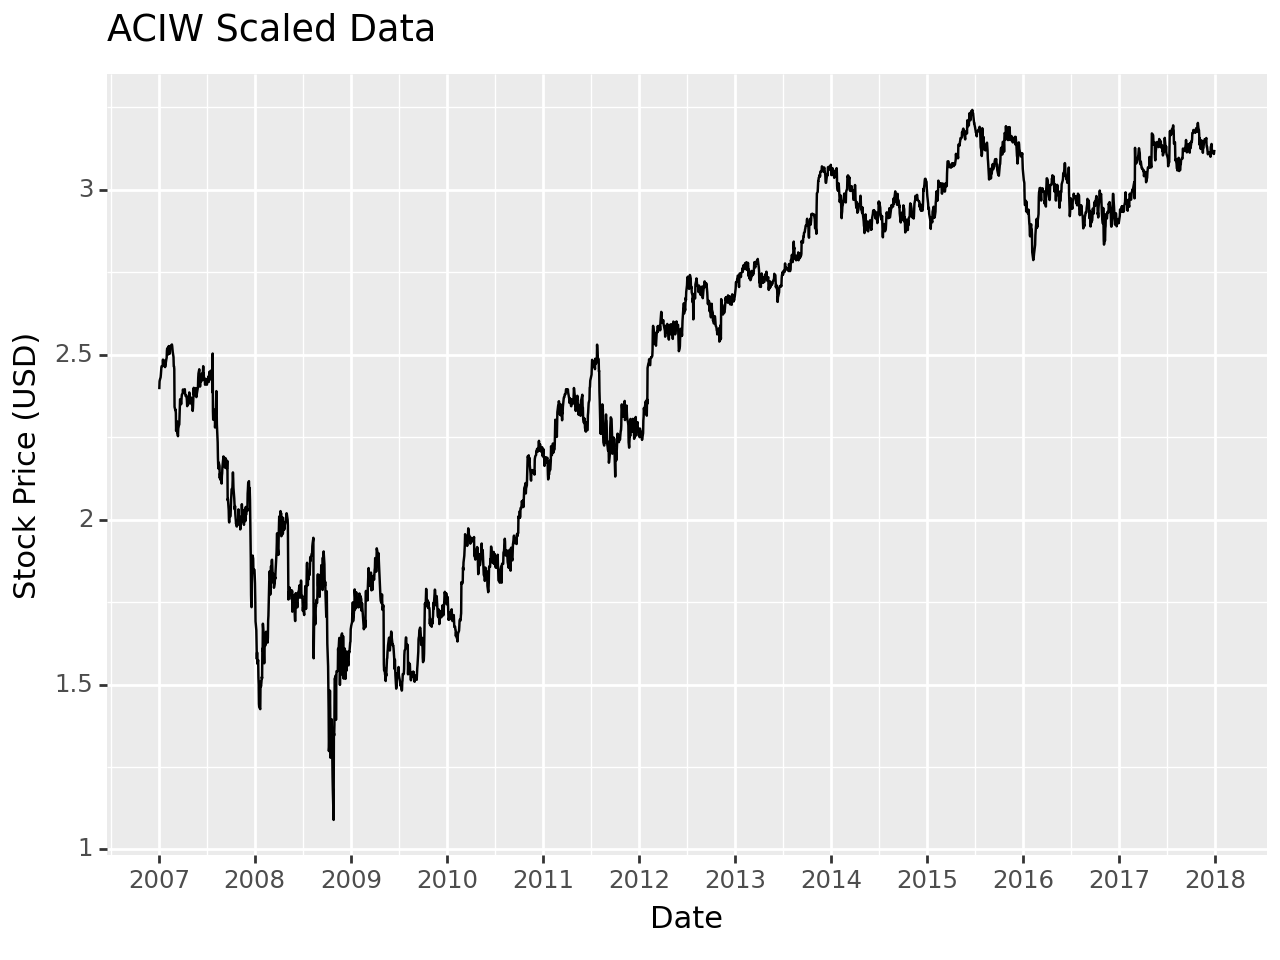
\includegraphics[width=0.7\linewidth]{images/aciw_scaled.png}
    \caption{Logged price data of ACIW Stock}
    \label{aciw_scaled}
\end{figure}

\begin{figure}[h]
    \centering
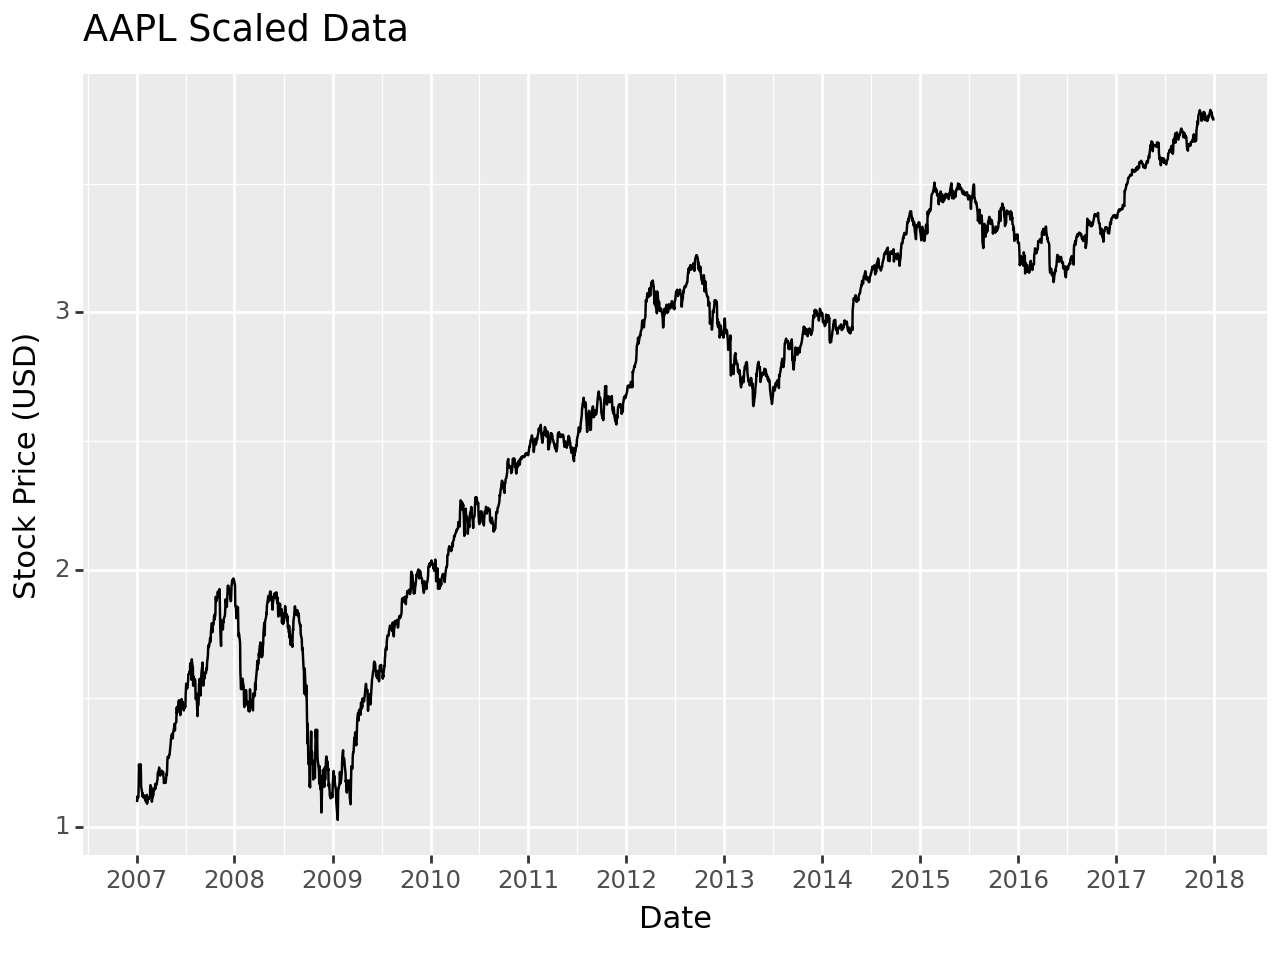
\includegraphics[width=0.7\linewidth]{images/appl_scaled.png}
    \caption{Logged price data of APPL Stock}
    \label{appl_scasled}
\end{figure}

\end{document}

